\subsection{Initial Testing} \label{methods:initial_testing}
Before delving into the GPU accelerated methods used to produce the final GKAGE product, we will here describe an initial test we performed in order to assess two things. Firstly, whether we could effectively GPU accelerate existing NumPy solutions using CuPy, all while staying within the comfort of Python, and secondly, whether such an implementation would result in significant speedup over a CPU solution or at least provide insight into how plausible getting significant speedup by utilizing the GPU was.
For this, we decided on focusing on the \textit{partial} \textit{k}mer counting problem, detailed in section \ref{background:kmers_and_kmer_counting}.

As detailed in section \ref{background:implementation_tools_and_libraries:npstructures}, npstructures is a Python library that enhances the NumPy library by providing additional data structures with NumPy-like behaviour and performance, built on top of NumPy.
Additionally in section \ref{background:implementation_tools_and_libraries:npstructures}, we detailed a subset of npstructures' data structures, one of which was a counter object that efficiently counts occurences of a predefined keys-set in a sample.
This counter object had previously been utilized to count a predefined set of \textit{k}mer's frequencies, albeit on the CPU.

Since npstructures' data structures are all heavily reliant upon NumPy's array routines for fast performance, they are designed around utilizing the CPU's vectorization and data parallelism.
Large array operations where data parallelism matters are ideal for the GPU architecture, which often can provide orders of magnitude more parallelism this way.
In addition, we know that most, if not all of the functionality used from NumPy, will be supported with GPU acceleration by CuPy through an nearly identical interface.
Thus, by replacing the NumPy functionality used in npstructures' data structures with CuPy's equivalent GPU accelerated functionality, we can GPU accelerate the necessary data structures in npstructures without having to leave Python.
With this strategy we GPU accelerated npstructures' counter object using CuPy.

\subsubsection{Using CuPy as a Drop-In Replacement for NumPy} \label{methods:initial_testing:using_cupy_as_a_drop_in_replacement_for_numpy}
Rather than creating a standalone package version of npstructures with GPU acceleration, we instead opted to add the possibility for GPU acceleration to the already existing package.
This added a new self imposed requirement; we did not want CuPy to be a npstructures dependancy since many users may wish to use it simply for the NumPy implementations.
Additionally, we still needed a way to redirect NumPy function calls to their equivalent CuPy functions.
We fulfilled both of these requirements by exploiting Python's module system.

Consider the following Python package example where our package, \textit{mypackage}, contains two modules, \textit{my\_classes} and \textit{my\_funcs}, both relying on NumPy for their implementations:

\begin{center}
mypackage.my\_funcs.py
\end{center}
\begin{lstlisting}[language=Python,style=pycode]
import numpy as np

def some_func_using_numpy():
  return np.zeros(10)
\end{lstlisting}

\begin{center}
mypackage.my\_classes.py
\end{center}
\begin{lstlisting}[language=Python,style=pycode]
import numpy as np

class SomeClassUsingNumPy:
  def __init__(self):
    self.data = np.zeros(10)

  def get_data(self):
    return self.data
\end{lstlisting}

Our package's initialization file imports our function and our class from their respective modules, and all functionality is usable without needing to import CuPy in either module or initialization file.
Pay attention to the initialization file's \textit{set\_backend} function which takes a library as a parameter and reassigns the np variable in both package modules from the NumPy to the provided library.

\begin{center}
mypackage.\_\_init\_\_.py
\end{center}
\begin{lstlisting}[language=Python,style=pycode]
from .my_funcs import some_func_using_numpy
from .my_classes import SomeClassUsingNumPy 

# Swaps NumPy with lib (presumably CuPy)
def set_backend(lib):
  from . import my_funcs
  my_funcs.np = lib

  from . import my_classes
  my_classes.np = lib
\end{lstlisting}

In our own program, where we will import our package, \textit{mypackage}, we can either directly use our package's implementation with NumPy, or we can do as the following example shows and import CuPy and set the backend in the entire package to use CuPy functionality instead of NumPy.

\begin{center}
program.py
\end{center}
\begin{lstlisting}[language=Python,style=pycode]
import cupy as cp

import mypackage
mypackage.set_backend(cp)

array = mypackage.some_func_using_numpy()
type(array) # cupy.ndarray
\end{lstlisting}

Exploiting Python's module system this way has the benefits of not making CuPy a dependancy for npstructures, and it also allows for gradual GPU support by way of only updating the backend in modules where the existing implementations are ready to be ported as is to CuPy.

\subsubsection{Resolving Unsupported or Poorly Performing Functionality}
Two issues can arise when utilizing this method of GPU accelerating NumPy code.
Firstly, some NumPy solutions may be effective on the CPU's architecture but ineffective on the GPU's, resulting in poor performance.
This will often be the case when significant portions of the code needs to be ran in a serial fashion, as opposed to parallel, or when array sizes are too small to mask the overhead of copying data to and from the GPU memory.
Secondly, certain NumPy functions are simply not supported by CuPy.
In case of the former issue, one might want to create an alternative solution that better utilizes the GPU's strengths, such as its massive parallelism.
For the latter issue, there is no other practical option than to create a custom solution that achieves the desired behaviour by using what CuPy functionality is available.
We circumvented both of these issues by creating custom implementations where we had the freedom to use the full extend of CuPy's functionality to reproduce the desired behaviour.
For classes, this can be achieved by subclassing and overriding methods where we wish to create our new custom implementations.
To demonstrate this, we will have to slightly edit our example package, \textit{mypackage}.

Consider if our package's class definition had instead been the following:
\begin{center}
mypackage.my\_classes.py
\end{center}
\begin{lstlisting}[language=Python,style=pycode]
import numpy as np

class SomeClassUsingNumPy:
  def __init__(self):
    self.data = np.zeros(10)

  def pad_with_ones(self):
    arr = self.data
    self.data = np.insert(arr, [0, len(arr)], 1)
\end{lstlisting}

In the code above, we use NumPy's insert function, which as of April 2023 is not supported by CuPy.
To circumvent this issue, we can subclass our \textit{SomeClassUsingNumPy} class and create our own custom implementation of \textit{pad\_with\_ones}.
We will create a new file where we implement our CuPy compatible solution, and our subclass will override the \textit{pad\_with\_ones} method.
\begin{center}
mypackage.cp\_my\_classes.py
\end{center}
\begin{lstlisting}[language=Python,style=pycode]
import numpy as np
import cupy as cp

from .my_classes import SomeClassUsingNumPy

class CPSomeClassUsingNumPy(SomeClassUsingNumPy):
  def pad_with_ones(self):
    arr = self.data
    self.data = cp.pad(arr, (1, 1), 'constant', constant_values=1)
\end{lstlisting}

In the above example we override the \textit{pad\_with\_ones} method with our alternative implementation that uses a different CuPy function that is supported by CuPy, the \textit{pad} function.
Now, our two different \textit{pad\_with\_ones} implementations will behave equivalently, although our custom implementation will leverage CuPy and be GPU accelerated.

Finally, we need to make one small change to our package's initialization file so that users of our package will import our CuPy compatible subclass of \textit{SomeClassUsingNumPy} after setting the backend to CuPy:
\begin{center}
mypackage.\_\_init\_\_.py
\end{center}
\begin{lstlisting}[language=Python,style=pycode]
from .my_funcs import some_func_using_numpy
from .my_classes import SomeClassUsingNumPy 

# Swaps NumPy with lib (presumably CuPy)
def set_backend(lib):
  from . import my_funcs
  my_funcs.np = lib

  from . import my_classes
  my_classes.np = lib

  # Use CuPy compatible version of SomeClassUsingNumPy
  global SomeClassUsingNumPy
  from .cp_my_classes import CPSomeClassUsingNumPy
  SomeClassUsingNumPy = CPSomeClassUsingNumPy
\end{lstlisting}

By utilizing this method, we implemented partial GPU support for the npstructures library, including enabling GPU support for the counter object used to count occurences of a predefined key-set in a sample.

\subsubsection{Assessment} \label{methods:initial_testing:assessment}
To assess the effect GPU accelerating npstructures by using CuPy as a drop-in replacement for NumPy, we benchmarked the GPU accelerated npstructures counter object by counting the occurences of a predefined set of 50 million unique \textit{k}mers in a set of 20 million DNA reads, each of length 150.
This benchmark used BioNumPy to read the FASTA file in chunks of 10 million bytes, 2-bit encode the reads and hash the valid \textit{k}mers before counting.
The time spent preparing each chunk was not included in the final measured runtime, since we were only interested in seeing the effects of GPU accelerating npstructures' counter object.
It is important to note that while this benchmark provided a good assessment of the speedup gained from GPU accelerating our counter, it omits the overhead of transferring each chunk of \textit{k}mers to the GPU in order to be counted by our GPU accelerated counter.
We justified the omission of this overhead because of two reasons.
Firstly, during our initial testing we were only interested in assessing the runtime differences during processing on the GPU versus the CPU when using CuPy as a drop-in replacement for NumPy.
Secondly, we only GPU accelerated one component of a much larger pipeline, and in such a case, the true effects of GPU acceleration may be overshadowed.
Our intention was to GPU accelerate several consecutive components in a way where only a single copy step would need to be performed before several consecutive processing steps could benefit from GPU acceleration, minimizing the effects of the CPU to GPU copy overhead.

\definecolor{cpucolor}{RGB}{255,255,225}
\definecolor{gpucolor}{RGB}{225,255,255}

\begin{figure}[H]
\begin{center}
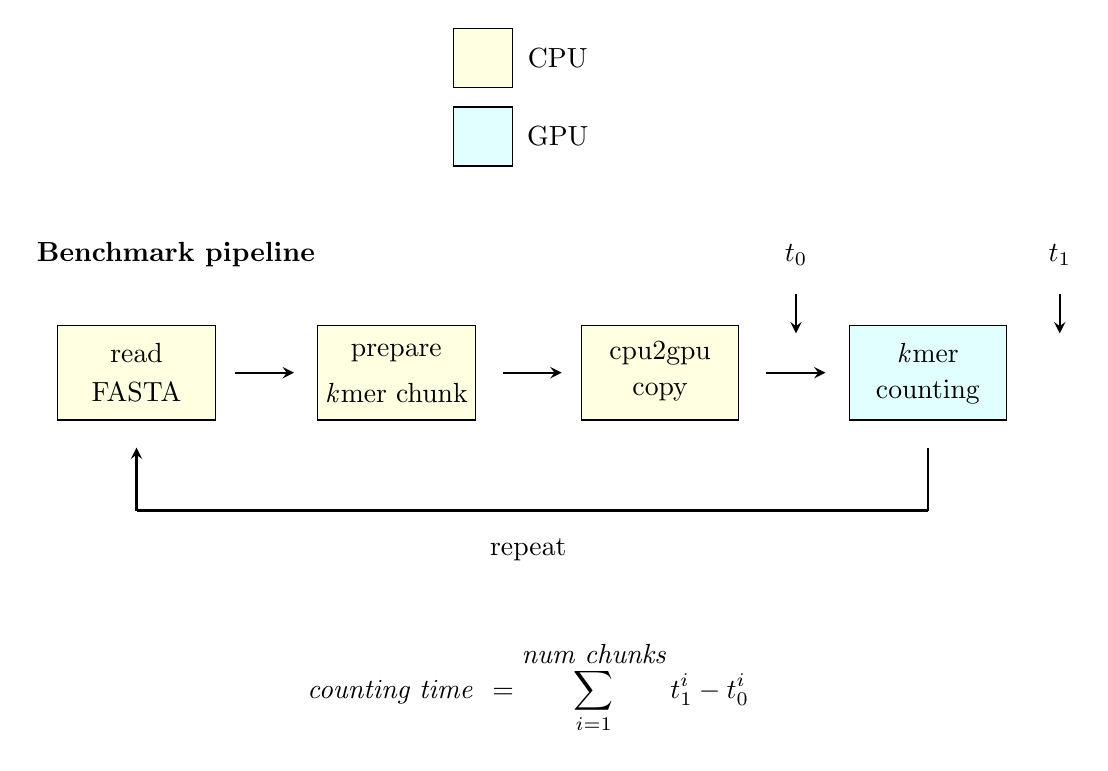
\begin{tikzpicture}
  \node at(5.35,-1)[]{\smaller{CPU}};
  \node at(5.35,-2)[]{\smaller{GPU}};
  \node at(4.4,-1)[draw,minimum width=.75cm,minimum height=.75cm,fill=cpucolor]{};
  \node at(4.4,-2)[draw,minimum width=.75cm,minimum height=.75cm,fill=gpucolor]{};
  % -- GPU --
  \node at(.5,-3.5)[]{\smaller{\textbf{Benchmark pipeline}}};
  % read fasta
  \node at(0,-5)[draw,minimum width=2cm,minimum height=1.2cm,fill=cpucolor](start){};
  \node at(0,-4.75)[]{\smaller{read}};
  \node at(0,-5.25)[]{\smaller{FASTA}};
  \draw [thick,-stealth](1.25,-5) -- (2,-5);
  % 2-bit encoding
  \node at(3.3,-5)[draw,minimum width=2cm,minimum height=1.2cm,fill=cpucolor]{};
  \node at(3.3,-4.75)[]{\smaller{prepare}};
  \node at(3.3,-5.25)[]{\smaller{\textit{k}mer chunk}};
  \draw [thick,-stealth](4.65,-5) -- (5.4,-5);
  % kmer hashing
  \node at(6.65,-5)[draw,minimum width=2cm,minimum height=1.2cm,fill=cpucolor]{};
  \node at(6.65,-4.75)[]{\smaller{cpu2gpu}};
  \node at(6.65,-5.25)[]{\smaller{copy}};
  \draw [thick,-stealth](8,-5) -- (8.75,-5);
  % cpu2gpu copy
  \node at(10.05,-5)[draw,minimum width=2cm,minimum height=1.2cm,fill=gpucolor]{};
  \node at(10.05,-4.75)[]{\smaller{\textit{k}mer}};
  \node at(10.05,-5.25)[]{\smaller{counting}};
  %\draw [thick,-stealth](11.4,-5) -- (12.05,-5);
  % arrows
  \draw [thick](10.05,-5.95) -- (10.05,-6.75);
  \draw [thick](10.05,-6.75) -- (0,-6.75);
  \draw [thick,-stealth](0,-6.75) -- (0,-5.95);
  \node at(4.975,-7.25)[]{\smaller{repeat}};
  % timestamps
  \draw [thick,-stealth](8.375,-4) -- (8.375,-4.5);
  \draw [thick,-stealth](11.725,-4) -- (11.725,-4.5);
  \node at(8.375,-3.5)[]{\smaller{$t_0$}};
  \node at(11.725,-3.5)[]{\smaller{$t_1$}};

  \node at(4.975,-9)[]{\textit{counting time}$\hspace{.65em}=\displaystyle\sum_{i=1}^{\textit{num chunks}}t_1^i - t_0^i$};

\end{tikzpicture}
\end{center}
\caption{
  The pipeline used to benchmark the CuPy-based against the NumPy-based npstructures counter object.
  Only the calls made to the counter object to count chunks of \textit{k}mers are timed, and these times are finally summed to get the total runtime spent on counting \textit{k}mers.
  The difference between the two runtimes are then used to infer the effects of GPU accelerating npstructures' counter object using our initial testing method.
}
\label{methods:initial_testing:figures:benchmark_overview}
\end{figure}

We ran the \textit{k}mer counting pipeline and measured the time spent counting \textit{k}mers for both the NumPy-based CPU version of the counter and the CuPy-based GPU version.
The total time spent counting \textit{k}mers was measured by timing each call to the counter object and summing these runtimes in order to get the total counting time.
For the GPU version, we made sure to synchronize the GPU to the CPU between each call, since kernel calls made from the CPU to the GPU are asynchronous otherwise.
This benchmark yielded the following results: 

\begin{table}[H]
\begin{center}
\begin{tabular}{lllll}
\multicolumn{1}{l|}{\textbf{Method}} & \multicolumn{1}{l}{\textbf{Counting time (seconds)}} &  \\ \cline{1-2}
\multicolumn{1}{l|}{NumPy} & \multicolumn{1}{l}{234.7} &  \\
\multicolumn{1}{l|}{CuPy} & \multicolumn{1}{l}{24.31}
\end{tabular}
\end{center}
\caption{
  The total time spent counting \textit{k}mers using npstructures' counter object, one with NumPy as the backend array-library, running on the CPU using one thread, and the other using CuPy as the backend, running on the GPU.
}
\label{methods:initial_testing:tables:benchmark}
\end{table}

\begin{figure}[H]
\hspace*{7em}
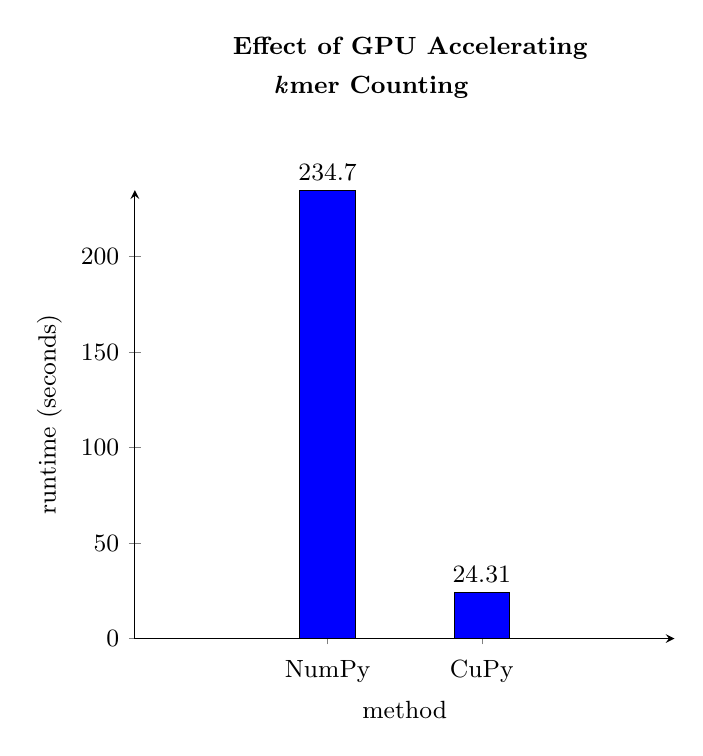
\begin{tikzpicture}[font=\small]
  \pgfplotsset{
    compat=newest,
    xlabel near ticks,
    ylabel near ticks
  }
  \pgfplotsset{compat=1.11,
      /pgfplots/ybar legend/.style={
      /pgfplots/legend image code/.code={%
         \draw[##1,/tikz/.cd,yshift=-0.25em]
          (0cm,0cm) rectangle (3pt,0.8em);},
     },
  }
  \node at(3.5,7.5)(){\textbf{Effect of GPU Accelerating}};
  \node at(3,7)(){\textbf{\textit{k}mer Counting}};
 
\begin{axis} [
  ylabel={runtime (seconds)},
  xlabel={method},
  ybar,
  bar width=20pt,
  ymin=0,
  xtick=data,
  axis x line=bottom,
  axis y line=left,
  enlarge x limits=1.25,
  symbolic x coords={NumPy, CuPy},
  xticklabel style={anchor=base, yshift=-\baselineskip},
  /pgf/number format/.cd,fixed,precision=3,
  nodes near coords={\small\pgfmathprintnumber{\pgfplotspointmeta}},
  legend style={anchor=west},
]

\addplot[fill=blue] coordinates {
    (NumPy, 234.7)
    (CuPy, 24.31)
};
\end{axis}
\end{tikzpicture}
\caption{
  Elapsed time counting the occurences of 50 million unique \textit{k}mers in a set of 20 million reads, each of 150 bases.
  Both methods use BioNumPy to read, 2-bit encode and hash chunks of \textit{k}mers, reading 10 million byte chunks from the FASTA at a time.
  Both methods also use npstructures' NumPy-based counter object to count the \textit{k}mer frequencies, although the CuPy-based version replaces NumPy with CuPy to achieve GPU acceleration.
}
\label{methods:initial_testing:figures:benchmark}
\end{figure}

As can be seen in table \ref{methods:initial_testing:tables:benchmark}, simply using CuPy as a drop-in replacement for NumPy in npstructures to GPU accelerate its counter object yielded a nearly 10X speedup in counting efficiancy, without having to otherwise change the implementation or even leave Python.
